\section{Empirical Results}
\label{sec:empirical-results}
To evaluate the algorithms presented in Section~\ref{sec:flexible-resource-allocation-mechanisms},
this section analyses the performance of both the greedy and auctions algorithms
(subsections~\ref{subsec:evaluation-of-the-greedy-algorithm} and~\ref{subsec:evaluation-of-the-auction-mechanisms}).
We investigate the effect of server heuristics on the Decentralised Iterative Auction
(subsection~\ref{subsec:effectiveness-of-decentralised-iterative-auction-heuristics}) and
the possibility of misreporting task attributes within the Decentralised Iterative Auction
(subsection~\ref{subsec:possibility-of-misreporting-task-attributes-in-decentarlised-iterative-auction}).
Finally we analyse the effectiveness of elastic resource allocation given server resource capacity ratios
(subsection~\ref{subsec:the-effective-of-elastic-resources-given-server-resource-capacity-ratio})
and the comparison between online and batched resource allocation
(subsection~\ref{subsec:comparison-between-online-and-batched-resource-allocation}).

Within Edge Cloud Computing, we have found no de facto standard for testing resource allocation algorithms and
those used in related work do not consider a deadline applicable for our work. Therefore we have generated synthetic
models for our servers and tasks. This is done using a handcraft Gaussian distribution for each attribute (this can be
found in Appendix~\ref{}). %% TODO

In order to compare the results of the difference algorithms, a branch and bound solution was implemented to solve
the optimisation problem, from section~\ref{subsec:optimisation-problem}, optimally. However due to the difficulty of
finding the optimally solution, this solution was only used in small settings tested. \\
For comparing to previous work with a fixed resource requirement, the minimum total resource required to run a task
within its deadline was found. These speeds were then used as the resource speeds of the task giving each task an
balanced amount of each resource. This is believed to be the best case as some tasks may required an extremely
unbalanced amount of resource.

\subsection{Evaluation of the Greedy Algorithm}
\label{subsec:evaluation-of-the-greedy-algorithm}
Using the optimal solution, as described above, the greedy solution can be compared to both the flexible resource
allocation optimal social welfare solution and the fixed resource allocation optimal solution. As well as this, a
relaxed version of the problem was implemented as an upper bound. This was done by combining all of the servers into
a single server with the combined resource capacity. \\
To implement the greedy mechanism, the value density function is $\frac{v_j \cdot d_j}{s_j + w_j + r_j}$, server selection
is $\text{argmin}_{\forall i \in I} S^{'}_i \cdot W^{'}_i \cdot R^{'}_i$ for task $j$ and servers $I$ and the resource
allocation is $\text{argmin}_{s^{'}_j, w^{'}_j, r^{'}_j} \left(\frac{w^{'}_j}{W^{'}_i}\right)^3 + \left(\frac{s^{'}_j + r^{'}_j}{R^{'}_i}\right)^3$
is task $j$ and server $i$.

\begin{figure}
    \centering
    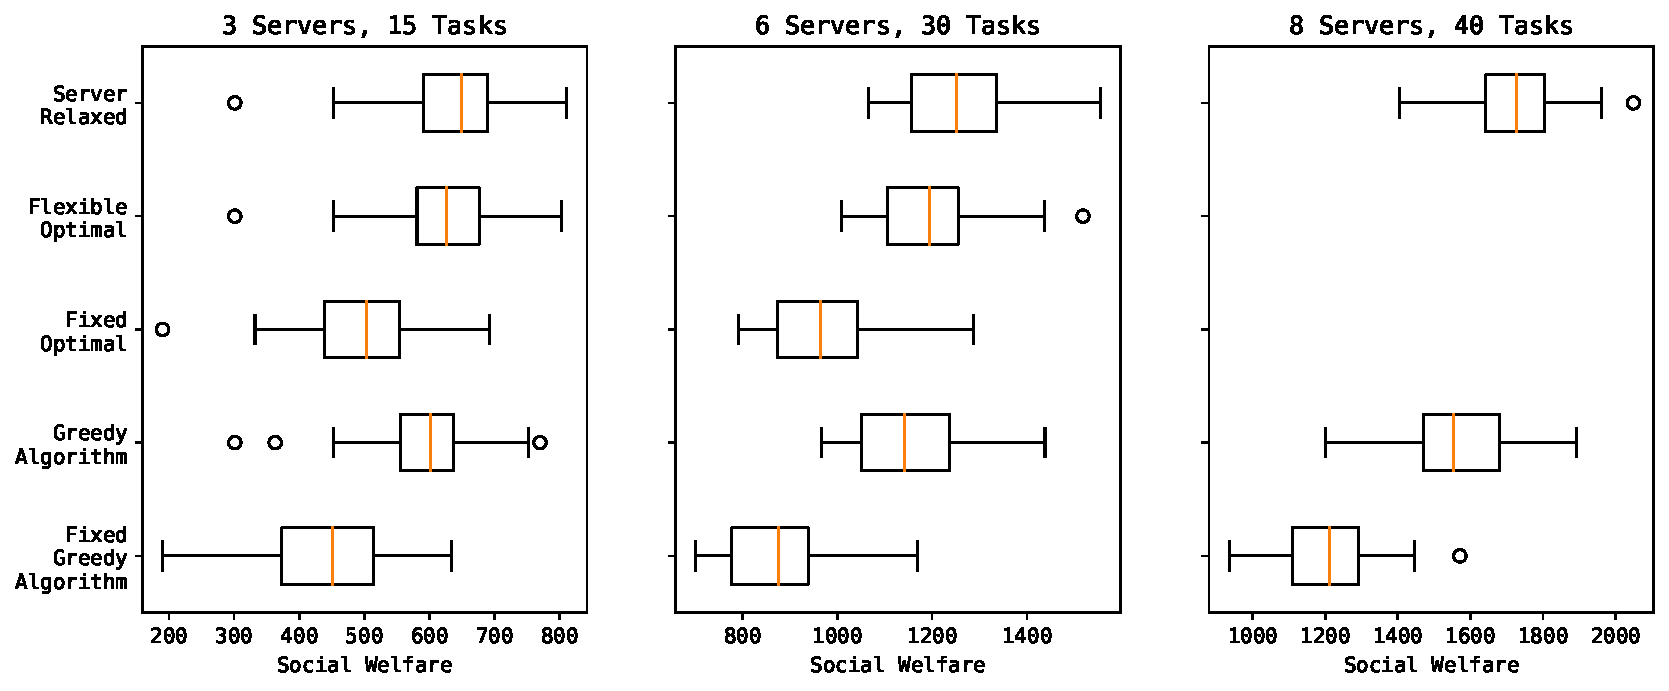
\includegraphics[width=\linewidth]{figs/greedy/multi_setting_social_welfare.pdf}
    \caption{Percentage difference in social welfare per model between greedy mechanism, flexible optimal solution,
             optimal server relaxed solution, fixed optimal solution}
    \label{fig:greedy-mechanism-comparison}
\end{figure}
%% TODO add percentage difference of the results
As figure~\ref{fig:greedy-mechanism-comparison} shows, the greedy mechanism achieves 98\% of the optimal solution for
the small models, the mechanism achieves within 95\% for larger models. In comparison, the fixed allocation achieves
80\% of the optimal solution and always does worse than the social welfare of the greedy mechanism.

\subsection{Evaluation of the Auction mechanisms}\label{subsec:evaluation-of-the-auction-mechanisms}
VCG, as explained in section~\ref{sec:flexible-resource-allocation-mechanisms}, is the traditional method of dealing
with self-interested users due to being incentive compatible. However, this requires solving the optimal solution
for each individual task making such a mechanism infeasible except for small setting. Because of this, VCG is used for
a comparison with the Critical Value Auction and Decentralised Iterative Auction in the small setting.

\begin{figure}[h]
    \centering
    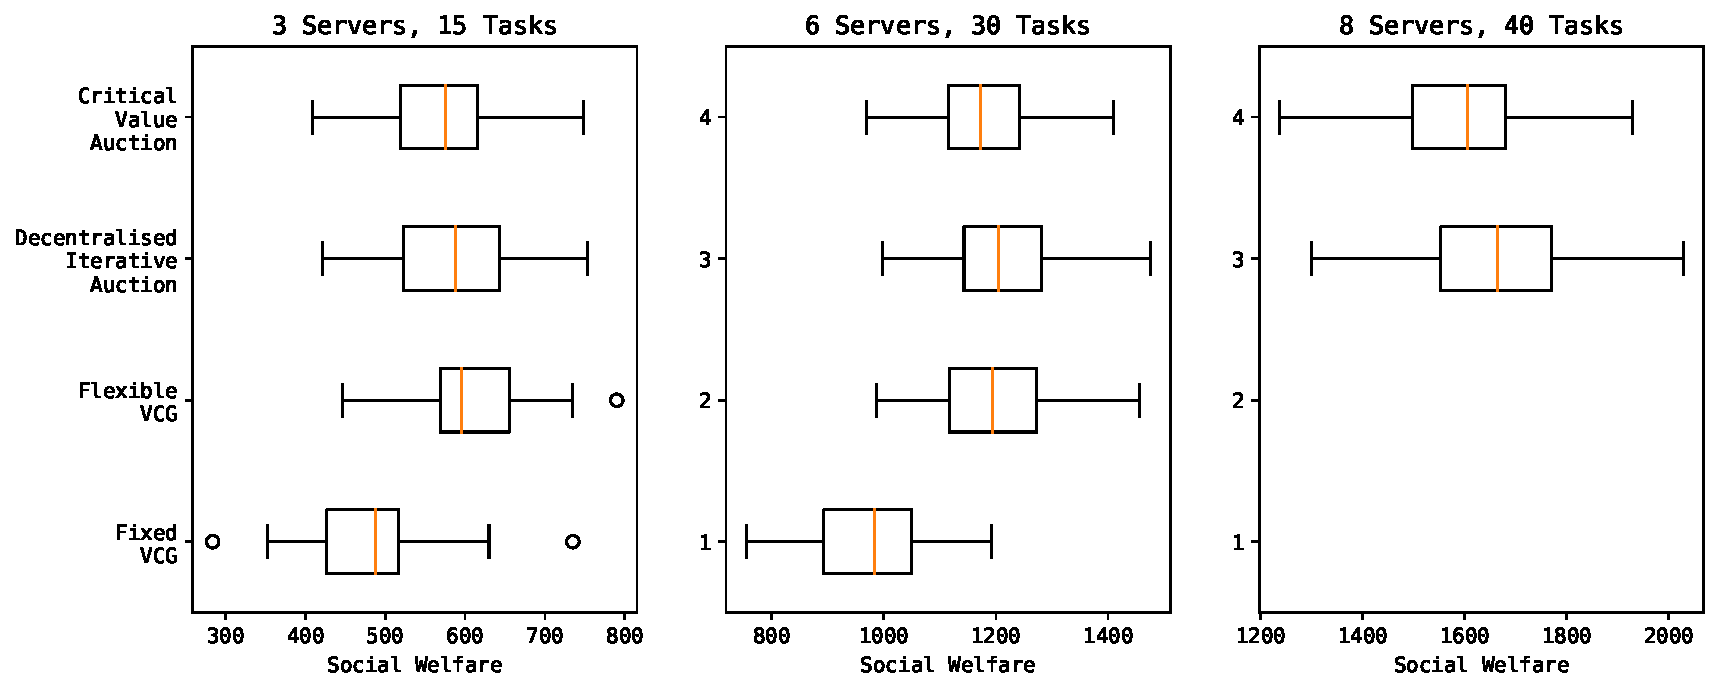
\includegraphics[width=\linewidth]{figs/auctions/multi_setting_social_welfare.pdf}
    \caption{Comparison of the social welfare for the auction mechanisms}
    \label{fig:auction-mechanisms-social-welfare}
\end{figure}

For the Critical Value Auction, the same modular functions as the greedy algorithm evaluated below are used, meaning
that the social welfare for the auction is identical to the greedy mechanism below. \\
For the decentralised iterative auction, the server heuristics used are a price change of 3 and an initial price of 25
for all servers. The reason for this selection of heuristics over others is explained in
subsection~\ref{subsec:effectiveness-of-decentralised-iterative-auction-heuristics}.

Figure~\ref{fig:auction-mechanisms-social-welfare} compares the social welfare of the auction mechanisms: VCG auction,
fixed resource speed VCG auction, critical value auction and the decentralised iterative auction.
Figure~\ref{fig:auction-mechanisms-revenue} compares the revenue instead.

\begin{figure}[h]
    \centering
    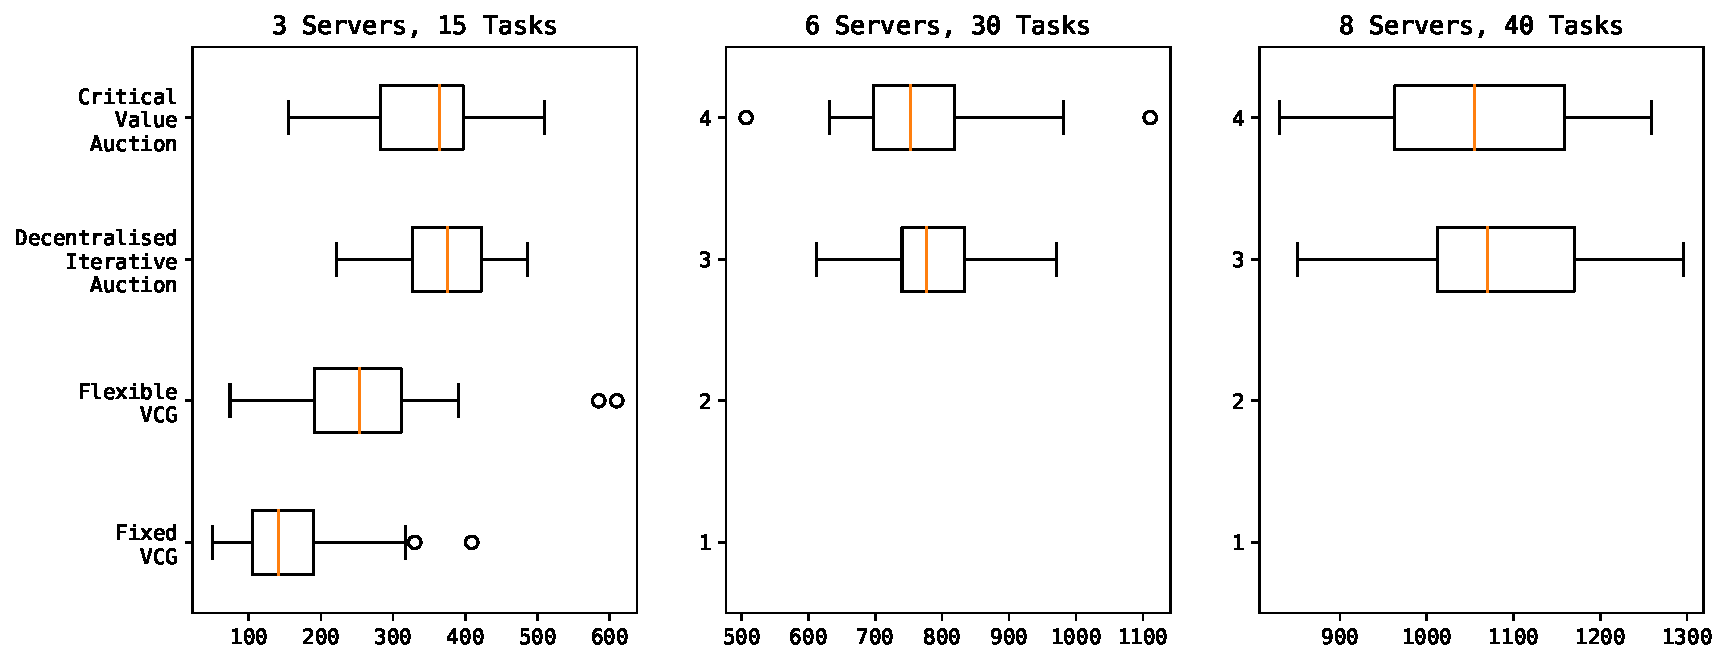
\includegraphics[width=\linewidth]{figs/auctions/multi_setting_revenue.pdf}
    \caption{Comparison of the social welfare for the auction mechanisms}
    \label{fig:auction-mechanisms-revenue}
\end{figure}
%% TODO add percentage difference of the results

\subsection{Effectiveness of Decentralised Iterative Auction Heuristics}
\label{subsec:effectiveness-of-decentralised-iterative-auction-heuristics}
As explained in subsection~\ref{subsec:decentralised-iterative-auction}, the price of task is calculated by the
Decentralised Iterative Auction through the difference in revenue between the task being allocated (with a price of
zero) and not being allocated. To increase a server revenue, a server will increase the price by a value referred to as
the price change variable. This is important as if a task has a value of 10 and the difference in revenue is 7 but the
price change is 4 then the resulting price is 11 above the task's value. As a result, the task won't be allocate to the
server however if the price change was 3 then the task could have been allocated resulting in the server's total
revenue benefiting both the server and the task in question. \\
A second heuristic, the initial price variable, is used to speed up the auction and reduce the number of rounds by
aiming to set the price close to the task's actual value. However, a similar problem as the price change variable exists
such that if a task's initial price is greater than the task's actual value then the task will never be allocated to a
task. \\
Therefore the selection of price change and initial price can have a significant impact on the social welfare, revenue
and number of rounds the auction takes.

Within the context of edge cloud computing, the number of rounds for the decentralised iterative auction is important
to making it a feasible auction as it is proportional to the time required to run. We investigated the effect of two
heuristic on the number of rounds and social welfare of the auction; the price change variable and initial cost
heuristic. With an auction using as minimum heuristic values for the price change and initial cost,
figure~\ref{fig:dia_rounds_grid_search}, on average 400 rounds were required for the price to converge while an auction
using a price change of 10 and initial cost of 20 means that only on average 80 rounds are required, 5x less. But by
using high initial cost and price change heuristics, this can prevent tasks from being allocated,
figure~\ref{fig:dia_sw_rev_grid_search}, shows that the difference in social welfare is only 2\% from minimum to
maximum heuristics.

\begin{figure}[h]
    \centering
    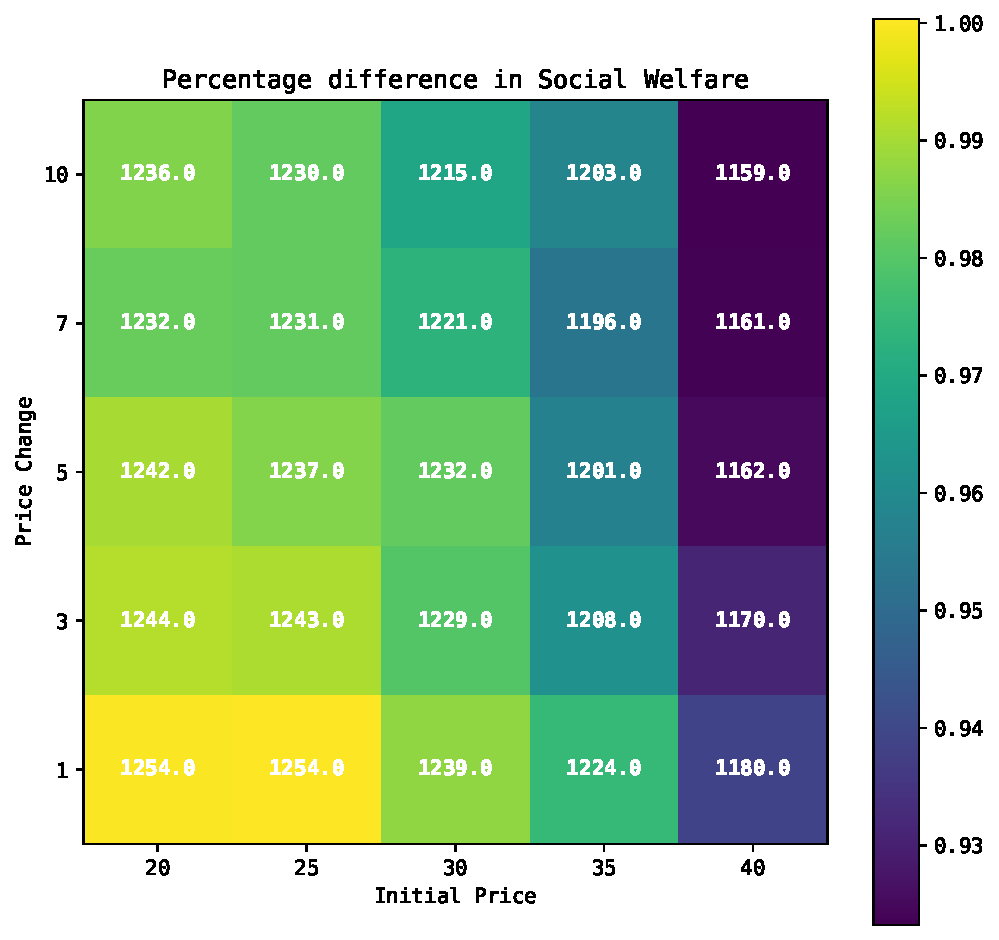
\includegraphics[width=0.45\linewidth]{figs/dia_heuristics/social_welfare_grid.pdf}
    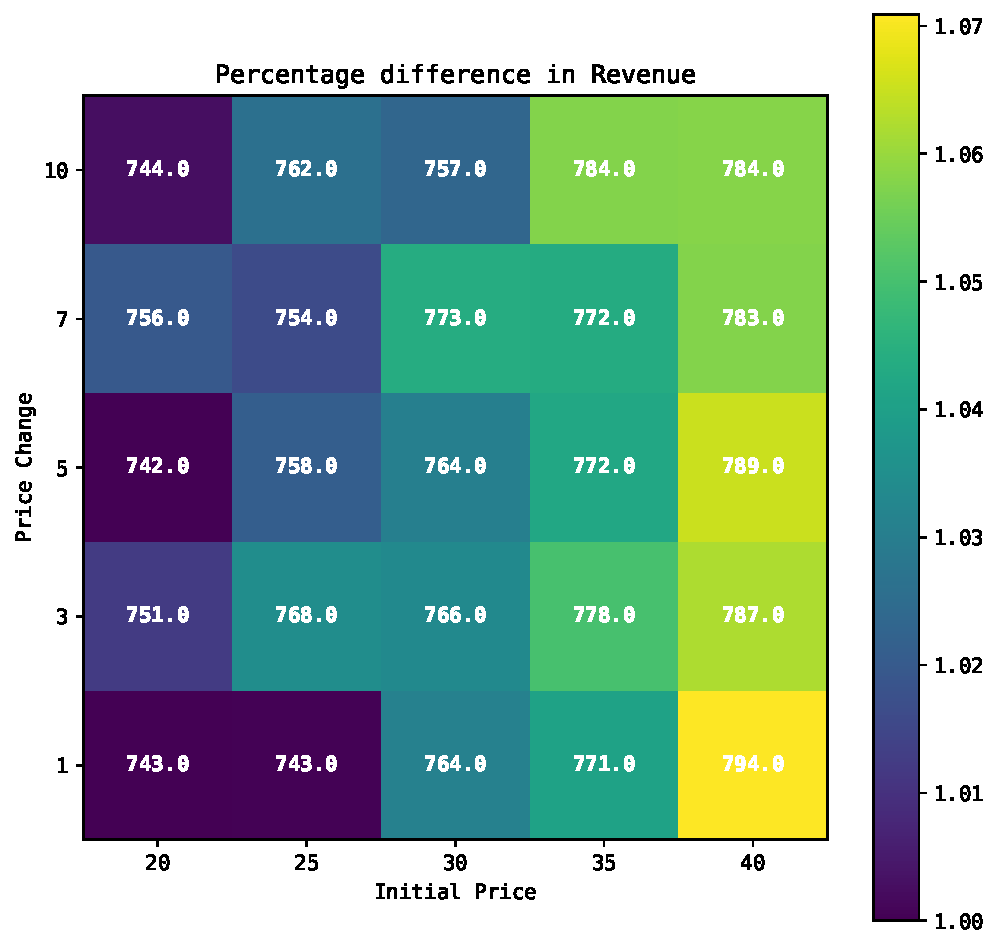
\includegraphics[width=0.45\linewidth]{figs/dia_heuristics/revenue_grid.pdf}
    \caption{Grid search of difference server price change and task initial cost effect on social welfare (left) and
             revenue (right)}
    \label{fig:dia_sw_rev_grid_search}
\end{figure}

\begin{figure}[h]
    \centering
    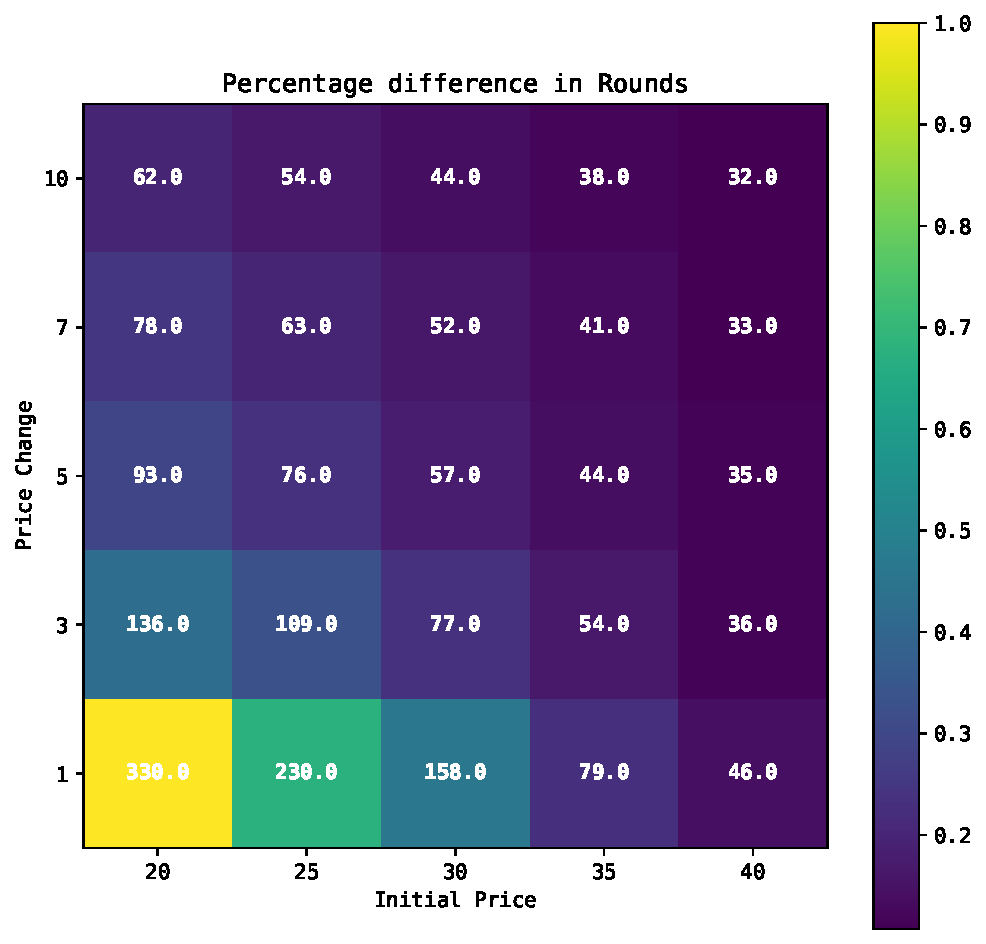
\includegraphics[width=0.45\linewidth]{figs/dia_heuristics/rounds_grid.pdf}
    \caption{Grid search of difference server price change and task initial cost effect on round count and number of
             task rounds}
    \label{fig:dia_rounds_grid_search}
\end{figure}

\subsection{The Possibility of Misreporting Task Attributes in Decentralised Iterative Auction}
\label{subsec:possibility-of-misreporting-task-attributes-in-decentarlised-iterative-auction}
In Subsection~\ref{subsec:decentralised-iterative-auction}, the Decentralised Iterative Auction was shown to be not
incentive compatible in specials cases however it is doubted that the ability for users to cheat more generally was
possible. Therefore, this problem was addressed by applying a grid search of task attributes and to randomly modify
individual tasks to investigate if tasks can pay less compared to if it didn't misreport.

For the random modification search, this was done by taking a random task and mutating each of the task's attributes.
For the deadline
% Explain the grid search
% Explain results

\subsection{The Effective of Elastic Resources given Server Resource Capacity Ratio}
\label{subsec:the-effective-of-elastic-resources-given-server-resource-capacity-ratio}
The major advantage of using elastic resource allocation is to the control that it gives to servers. This becomes
increasing important if task requirements are unbalanced compared to server resource capacity. To measure the impact
of elastic resource allocation compared to fixed resource allocation, server computation and bandwidth capacities
are redistributed to different ratios in order to compare. The reason only the computation and bandwidth capacities
are modified is due to the elasticity doesn't affect storage just the bandwidth (in loading and sending results,
eq~\ref{eq:server-bandwidth-constraint}) and computation (eq~\ref{eq:server-computation-constraint}). \\
Server resources are redistributed through using a percentage of the server's total (computation + bandwidth) resources.
This is shown as a ratio of server computation to bandwidth ratios in figures~\ref{fig:resource-ratio-social-welfare}
and~\ref{fig:resource-ratio-server-resource-usage}.

\begin{figure}[h]
    \centering
    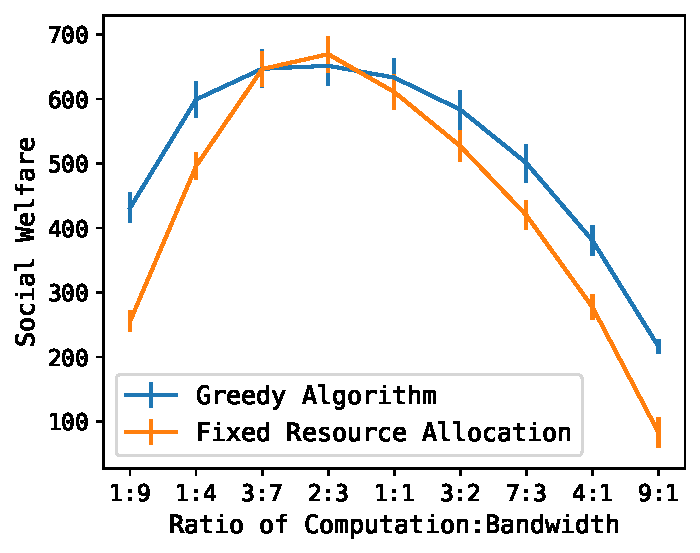
\includegraphics[width=0.45\linewidth]{figs/resource_ratio/social_welfare.pdf}
    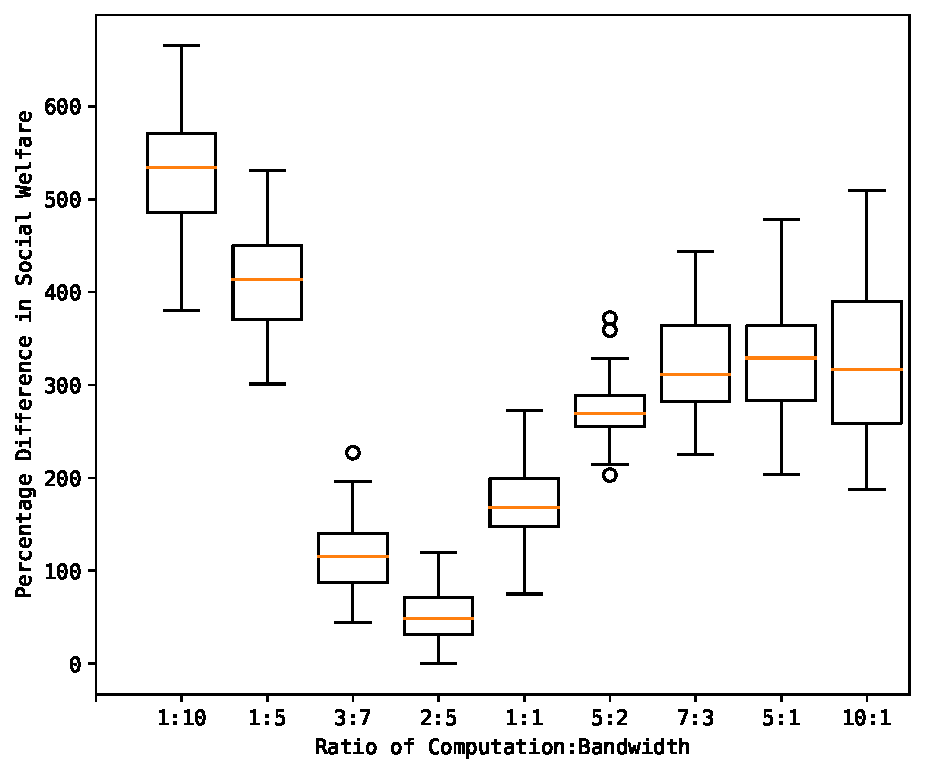
\includegraphics[width=0.45\linewidth]{figs/resource_ratio/social_welfare_difference.pdf}
    \caption{The effect of server resource ratios on average social welfare percentage and the social welfare difference}
    \label{fig:resource-ratio-social-welfare}
\end{figure}

Figure~\ref{fig:resource-ratio-social-welfare} is the combination of two graphs showing the same data. The left graph
shows the average social welfare achieved by the respective algorithms with different server resource ratios. At the
ratio extremes, there is a significant improvement in results. This can be seen more clear by the right graph, that
instead plots the difference in social welfare per model with the error bars. \\
This observation is important for Edge Computing as nodes may have a large discrepancy in server resource capacity
due to a persistence task running over a long period of time, internet connection issues limiting overall bandwidth,
etc. For these cases, the elasticity of tasks has a significant boost to the number of tasks and in social
welfare in comparison to fixed resource allocation.

\begin{figure}[h]
    \centering
    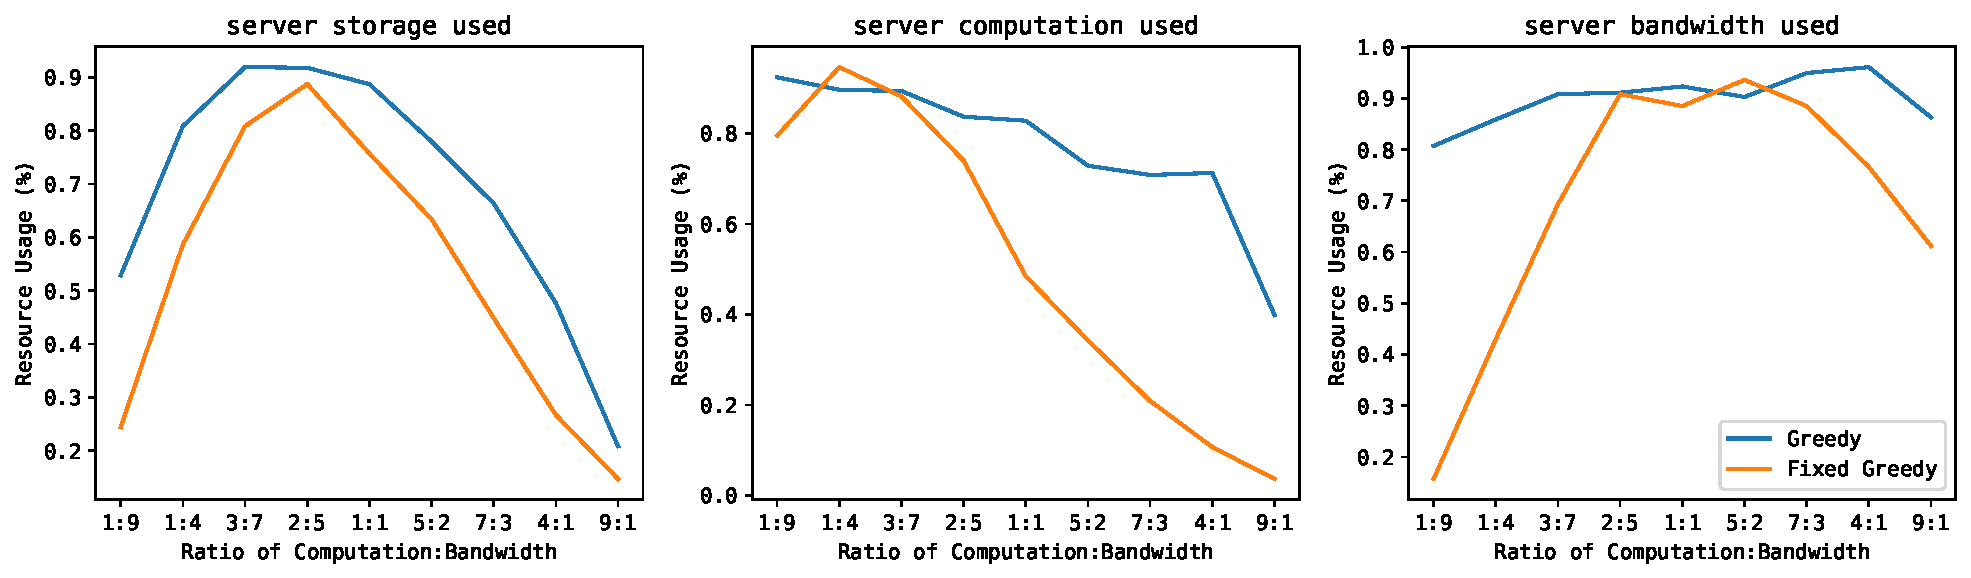
\includegraphics[width=\linewidth]{figs/resource_ratio/server_resource_usage.pdf}
    \caption{Server resource usage}
    \label{fig:resource-ratio-server-resource-usage}
\end{figure}

The effect of the redistribution of resources can be seen through the usage of resources by servers on average with
each ratio in figure~\ref{fig:resource-ratio-server-resource-usage}. For cases where there is a large capacity of a
resource available, for elastic resource allocation these resources are able to be used to maximise the number of tasks
that can be run. This is particularly true of bandwidth as for a majority of the ratios, it is limiting factor to be
able to allocate tasks.

\subsection{Comparison between Online and Batched Resource Allocation}
\label{subsec:comparison-between-online-and-batched-resource-allocation}
The purpose of this work has to be explore to use of elastic resource allocation in a static one-shot environment
meaning that all tasks arrive at the start which are then allocated. Section~\ref{sec:problem-formulation} proposed
that to deal with this problem that, in reality, task do arrive over time. The proposed algorithms could be modified
such that tasks are run in batches overtime. As a result, as tasks arrive they are added to a queue, waiting to be
allocated. So when a new batch occurs, all of the tasks in the queue can be processed using the proposed algorithms
with no modifications. \\
Therefore choosing the right branch length is important as the more competition means better selection of tasks
increasing social welfare while the longer the branch length reduces the length of the task processing time. For the
Decentralised Iterative Auction, it has an advantage practically of being run in a batch as the auction doesn't need to
wait for all of the tasks to arrive compared to the Critical Value Auction. Therefore the auction can run during the
batch time frame with the task allocation at the end of the batch being the allocation.

We choose the batch lengths: 1, 2, 3, 4 because the mean length of a task is 10, any longer than this would result in
tasks on average tasks having to be computed in half their possible time. Plus, as can be seen in
figure~\ref{fig:batch-task-allocation}, the total social welfare decreases as the batch lengths increase investigating
longer batch lengths unwarranted.

\begin{figure}
    \centering
    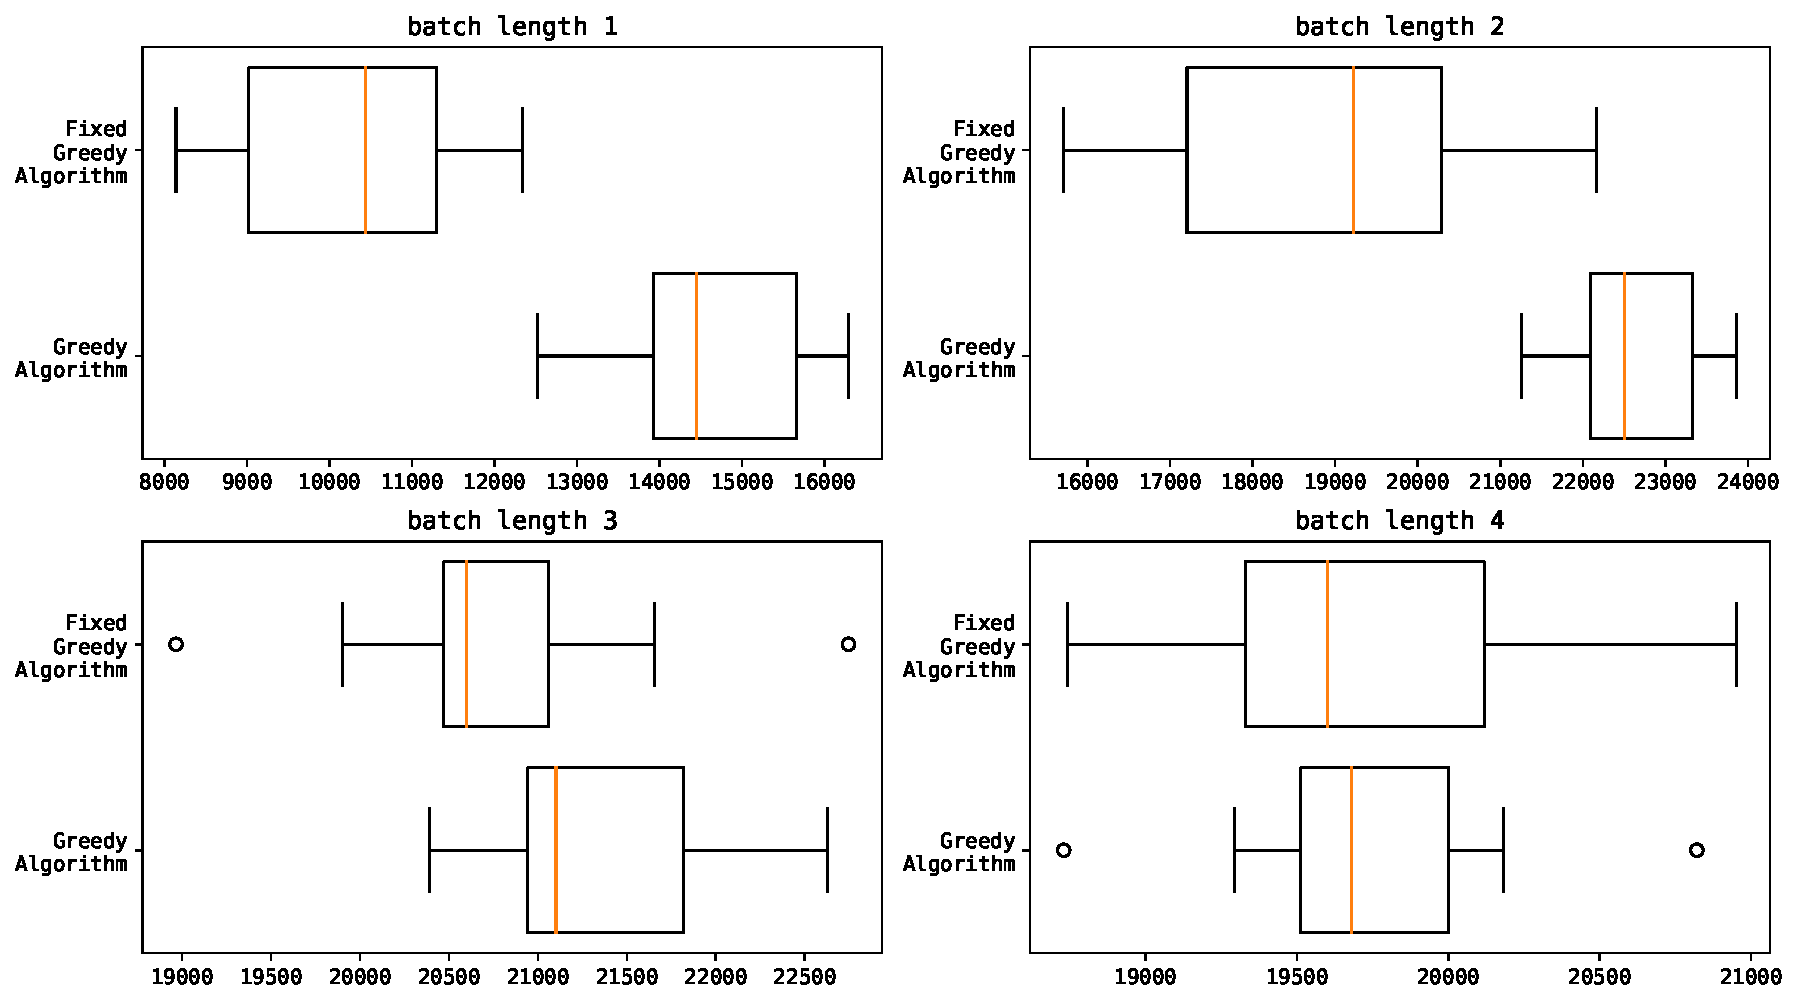
\includegraphics[width=\linewidth]{figs/online/online_batch_lengths.pdf}
    \caption{Online batch lengths}
    \label{fig:batch-task-allocation}
\end{figure}